% this file is called up by thesis.tex
% content in this file will be fed into the main document

\chapter{Design}\label{chap:methology} % top level followed by section, subsection
In this section we will look at the design of the system we used to test our research question: `What are the best mutation strategies of a coverage-guided fuzzer?'. To answer our question, we must first select a set of mutation strategies. Then we must select a set of metrics to determine how we will measure the performance of a strategy. Lastly we need a coverage-guided fuzzer. We have to run all of this on a set of binaries, so we will look at which binaries we need to pick. We also want to log metrics related to the condition which is being tested to see if we can find a correlation between a metric and a mutation strategy. We have designed a framework which will generate the results from the selected metrics and strategies, of which we will give a high level overview.

\section{Overview}\label{sec:overview}
A general overview of the framework is given in Figure \ref{fig:general}. We start with picking existing binaries with their source code. For these binaries, we also select some valid input seeds. The source code of the binary with the seeds is given to an existing coverage-guided fuzzer, which logs information about every condition hit in a trace. The source code is compiled by the fuzzer to insert their instrumentation. The output from the existing fuzzer is then passed as \texttt{(input, trace)} pairs from the fuzzer as input to the Fuzz Checker. The Fuzz Checker tries different mutation strategies for every condition in the trace, applied to the corresponding input. Hence, a \texttt{(input, condition)} pair is communicated to the strategies, which create a new mutated input and check if they flipped the condition against a specially instrumented version of the target binary, called the Oracle. 
During the process, data is gathered from several metrics which is combined in the output.
When the existing fuzzer is fuzzing the target program, we collect dynamic metrics for every condition.
The Fuzz Checker then calculates static metrics for the found conditions when obtaining the traces by recompiling the source code with an analysis pass.
When the result is obtained from the strategy, we obtain the microbenchmarks for the specific condition and strategy.
Once all runs are done, we extract the features from the data. For every condition, we calculate the label and the timing information. This information is passed to the machine learning models, to train the models an validate them and we generates statistics from this data.



\tikzset{app/.style={fill=yellow!20}}
\tikzset{ output/.style={fill=red!20, rounded corners=3pt}}
\tikzset{ code/.style={fill=blue!20, rounded corners=3pt}}
\tikzset{ input/.style={fill=green!20, rounded corners=3pt}}
\tikzset{ intermediate/.style={fill=gray!20, rounded corners=3pt}}
\begin{figure}[H]
    \centering
    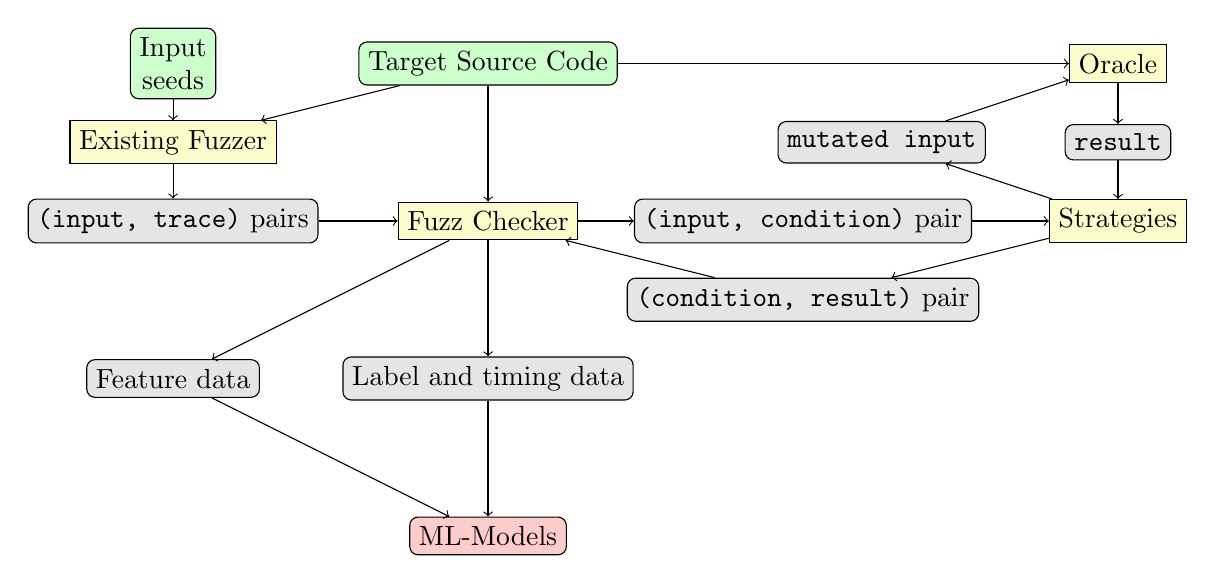
\begin{tikzpicture}[every node/.style={align=center}]
      % Dialectics
  \node[draw,input] (TargetSource) at (1,0) {Target Source Code};
  \node[draw,app] (ExistingFuzzer) at (-3,-1) {Existing Fuzzer};
  \node[draw,intermediate] (SymccCompiled) at (5,-3) {\texttt{(condition, result)} pair};
  \node[draw,input] (InputSeeds) at (-3,0) {Input\\ seeds};
  \node[draw,app] (SymccCompiler) at (9,-2) {Strategies};
  \node[draw,intermediate] (GeneratedInputs) at (-3,-2) {\texttt{(input, trace)} pairs};
  \node[draw,intermediate] (ConcolicInfo) at (5,-2) {\texttt{(input, condition)} pair};
  
  
  \node[draw,app] (Oracle) at (9,0) {Oracle};
  \node[draw,intermediate] (MutatedInput) at (6,-1) {\texttt{mutated input}};
  \node[draw,intermediate] (Result) at (9,-1) {\texttt{result}};
  
  \node[draw,app] (FuzzChecker) at (1,-2) {Fuzz Checker};
  \node[draw,intermediate] (Features) at (-3,-4) {Feature data};
  \node[draw,intermediate] (Label) at (1,-4) {Label and timing data};
  \node[draw,output] (OutputInformation) at (1,-6) {ML-Models};
  
 
  
  \draw[->] (TargetSource) to (ExistingFuzzer);
  \draw[->] (TargetSource) to (FuzzChecker);
  
  \draw[->] (TargetSource) to (Oracle);
  
  \draw[->] (SymccCompiler) to (SymccCompiled);
  
  \draw[->] (InputSeeds) to (ExistingFuzzer);
  
  \draw[->] (ExistingFuzzer) to (GeneratedInputs);
  
  \draw[->] (GeneratedInputs) to (FuzzChecker);
  \draw[->] (SymccCompiled) to (FuzzChecker);
  
  \draw[->] (FuzzChecker) to (ConcolicInfo);
  \draw[->] (ConcolicInfo) to (SymccCompiler);
  
  \draw[->] (SymccCompiler) to (MutatedInput);
  \draw[->] (Result) to (SymccCompiler);
  \draw[->] (Oracle) to (Result);
  \draw[->] (MutatedInput) to (Oracle);
  
  \draw[->] (FuzzChecker) to (Features);
  \draw[->] (FuzzChecker) to (Label);
  
  \draw[->] (Features) to (OutputInformation);
  \draw[->] (Label) to (OutputInformation);
  
  
    \end{tikzpicture}
    \caption{General overview of the architecture of the framework}
    \label{fig:general}
\end{figure}


\section{Picking Targets}
We start with picking some binaries on which we want to run our tests. We need to select binaries of which the source code is available, since we have to instrument them.
We want to create a dataset representing real world programs, so we try to select a diverse set of binaries. Since in \cite{lyu2019mopt} the authors explain that different mutation strategies differ in efficiency when fuzzing different applications, we wanted to have a broad collection of binaries, without artificial created execution paths, like in the LAVA-M dataset \cite{dolan2016lava}. The LAVA-M dataset contains bugs which are often triggered after a specific magic byte. Since these bugs are created artificially, we do not use this dataset. 

We found binaries in prior work on which they evaluated fuzzers, which are also used in real world settings.
We picked the following binaries:

\begin{itemize}
    \item \texttt{file}. We wanted to include a simple binary in our dataset, which mostly matches the input against a set of magic bytes.
    \item \texttt{jhead}. Another simple binary which parses header information of a \texttt{jpeg} file.
    \item \texttt{xmlwf}. This binary is a parser for xml files and uses the \texttt{libexpat} library.
    \item \texttt{tcpdump -nr}. This binary we used as a parser for pcap files and uses the \texttt{libpcap} library. The \texttt{n} argument disables the DNS lookup, which causes a large speed increase.
    \item \texttt{djpeg}. This binary is a decompression tool for jpeg files and uses the \texttt{libjpeg} library.
    \item \texttt{nm -C}. This binary parses other binaries and outputs the symbols from the binary. The \texttt{C} argument demangles low-level symbol names into user-level names. It is part of the \texttt{binutils} repository, which also includes other binaries like \texttt{objdump} and \texttt{size}. However, there is a lot of overlap in their code so we only used this binary from this repository, because it is used in prior work \cite{chen2018angora}. 
    \item \texttt{gif2png}. This binary is a conversion tool for gif images to png images and uses the \texttt{libpng} library. The newest version of \texttt{gif2png} is written in Go instead of C, so we used the latest version available in C.
    \item \texttt{tiff2pdf}. This binary is a conversion tool for tiff images to create pdf files and uses the \texttt{libtiff} library.
\end{itemize}
All of these binaries are common targets of prior work \cite{chen2018angora, she2019neuzz, han2019synfuzz, rawat2017vuzzer, yun2018qsym, liang2019deepfuzzer}.
For the exact versions and commit hashes of the used binaries see Appendix \ref{appendix:repos}.
\section{Existing fuzzer}
To collect conditions from the selected binaries, we first need several execution traces of the selected binaries, which should contain some minimal information about every condition. We can collect the traces by using an existing coverage-guided fuzzer and modifying it, such that we can store and access each individual execution trace.
Because we want to look at conditions, and we mostly came up with the research question because of the Angora fuzzer, we decided to use this fuzzer as our starting point. Other advantages of this fuzzer where the fact that it uses 2 types of instrumentation, which we could use this as starting point for our Oracle, and it stores all dynamic taint information of a given trace already in a file. 
In Chapter \ref{chap:implementation} we will explain in detail what we modified.

A disadvantage from the collected dataset could be that the found traces contain more conditions which can be flipped by the gradient descent algorithm, since this mutator is present in the Angora fuzzer. However, this will be the case for any tried mutator, for any fuzzer, since a fuzzer using random mutations could be biased towards conditions more easily flipped by random mutations.

%Angora uses 2 types of instrumentation to collect information from a binary. It has a fast variant and a track variant. In the track instrumentation, it uses the DataFlowSanitizer \cite{dataflowsanitizer} to instrument it with heavy dynamic taint tracking. This is used to collect a new trace if a new path in the program is found. These are the traces we want to collect for later analysis.

%The fast variant only has limited instrumentation. It inserts an extra check after every if or switch statement which is only triggered when this is the condition being targeted. It then registers this condition is true or false and logs this.

Once we have collected the traces, we have a mapping of \texttt{(input, trace)} pairs. Because we want to run our Fuzz Checker against many conditions, we try covering a large part of the conditions in the binary by giving the binaries at least one input seed which contains a format the binary is expecting. This is done because it is generally hard for a fuzzer to construct a valid input file from scratch \cite{you2019slf}.
All binaries are also given the string `\texttt{hello world}' as input seed.

We have decided to collect the traces in the existing fuzzer with context awareness, since in Angora \cite{chen2018angora} the authors suggest this leads to more program coverage. Our version of context awareness changes context on a function call. This means that the context of a condition is considered the same, only if the function call stack to reach that condition is the same.

We mark a condition as unique when the condition, context and the condition result are unique. We want to flip every condition both ways, therefore we also consider the condition result when looking at uniqueness. We then skip a condition if we have seen it before using the constructed uniqueness property. This is done to prevent the first conditions of a trace or common code paths to skew the results, since these are likely to be the same for all traces.


\section{Fuzz Checker}
The \texttt{(input, trace)} pairs are fed to the Fuzz Checker, together with the target source. In this module, we mutate every input with every strategy for every condition in the corresponding trace. We do this by communicating a \texttt{(input, condition)} pair to every strategy, where the input is the one from the \texttt{(input, trace)} pair, and the condition occurred in the trace. In the next section we will explain which strategies we used. When a strategy has mutated an input, it checks if it has flipped the condition by running it against the Oracle, because the Oracle tells us if we have flipped a specific branch by communicating it back to the framework. This gives us a \texttt{(condition, result)} pair. For every condition seen, we store which strategies flipped it with additional information depending on the strategy. Since we are not interested in the execution after the condition has been reached, we terminate the Oracle after the condition has been hit and store the time it took to flip the condition. The framework then collects the static metrics from the source code as explained in Section \ref{subsec:designStaticMetrics}. The framework also collects dynamic metrics from the traces as explained in Section \ref{subsec:designDynamicMetrics} and the microbenchmarks as explained in Section \ref{subsec:performanceMetrics}. The chosen metrics measure the complexity of a condition which relates to how hard it is to flip a condition. This data is then be used to create machine learning models as explained in Section \ref{sec:MLmodels}. 

%We have created two types of models.
%One model classifies, based on the collected metrics, if a condition is flippable or not. Such a model can be useful to a fuzzer to prioritise conditions.
%Another model uses regression to predict the time it takes for a strategy to flip a given condition, such that a fuzzer can select the fastest strategy.

%It will register if a condition is flipped given an input and communicate this back to the fuzzer. For this we have to compile all binaries again. Since we are not interested in the behaviour of the program after a condition was or was not flipped, we terminate the target binary as soon as we hit the condition.
%To communicate the obtained information back to the main program, we use unix sockets. In order to quickly spawn multiple processes, we use a forkserver and forkclient setup, which fork the process from a client, which keeps the memory footprint low and prevents copying a lot of code pages, since the code pages of the binary use a \texttt{copy on write} strategy. \todo{source}

%Because we also want to implement a concolic strategy, we compile every binary also with the Symcc compiler as explained in section\ref{subsec:symcc}, which we modified to also support a subset of symbolic bytes from an input file. It will then output several new inputs. These new inputs can then be checked to see if we flip the desired condition.


\section{Strategies}\label{sec:implement-strategies}
In this section we will explain in depth which strategies we have chosen to mutate the input and why. 
We selected existing strategies from other fuzzers including some state-of-the-art fuzzers as explained in Section \ref{sec:benchmarking}.
However, when we inspected the source code of the strategies, we often found a lot of extra `tricks' in these strategies. For example, the Length strategy in \cite{chen2018angora}, which makes an input longer or shorter, also tries, after the initial try, to append a number of line terminators at the end, in the hope to trigger some new behaviour.
The `MagicByte' strategy in \cite{chen2018angora}, which inserts the characters found with the dynamic taint analysis, tries the random strategy if it has failed. Also from \cite{chen2018angora} the Gradient Descent strategy, which in its pure form should use a gradient instead of partial derivatives, switches to partial derivatives when it is unable to flip a branch using the gradient. Then it repicks a new start point using a random mutator. This combination of strategies makes it harder to say which part of the strategy is in fact used to flip a condition.
This is why we have chosen to use a more `pure' version of the implemented strategies, without any of the extra `tricks', to have a better sense of which part of a strategy causes the most flips in a condition. In some strategies, we do have multiple substrategies, but then we log which substrategy we are trying when we find a flip.
The only strategy which we did not implement ourselves, but used by modifying an existing program, is the concolic strategy. In Chapter \ref{chap:implementation} we will explain how we modified the program.

We also wanted to test the mutations from the input-to-state correspondence strategy from Redqueen as explained in Section \ref{subsec:redqueen} to compare their performance. Since we already have access to dynamic taint analysis, we apply the mutations on the corresponding input bytes without using the input-to-state correspondence to guess on which bytes we have to apply the taint. %As explained above, we use Symcc to create a concolic strategy. In section \ref{sec:implement-strategies} we will explain how we implemented these strategies.

We will briefly explain what every strategy does.

\subsection{Random strategy}
With a random strategy, some random mutations are applied to the input. Since we also have dynamic taint information for some conditions, we can use this information to only randomise the bytes from the input which are being used to construct the value to compare. However, if this is not available, we have to randomize arbitrary bytes in the input. This strategy is one of the most used strategies in fuzzers \cite{aflfuzzer, fioraldi2020afl++, rawat2017vuzzer, chen2018angora}.
\paragraph{Random strategy without taint}
We start with a given input for a condition. Then we randomly mutate the input between 1 and 10 times. A random mutation is either an insertion of a random byte, a removal of a random byte or a bitflip in a random byte.
In the AFL fuzzer\cite{aflfuzzer} 11 different mutation strategies are used, but since these are already extensively researched in \cite{lyu2019mopt}, and we here try to trigger a specific branch instead of any branch, we do not use the mutation operators which change large parts of the input, like combining multiple seeds. Therefore also the choice of randomizing only up to 10 bytes, because we do not want to mutate the input to such an extend we no longer reach the condition.
We call this strategy `RandomStrategy'.
\paragraph{Random strategy with taint}
We start with a given input but with taint information. From the taint information, we know exactly which bytes create the value which is being compared in the branch. We randomise all these bytes with the intention to flip the branch.
We call this strategy `RandomTaintStrategy'.

\subsection{One byte strategy}
This deterministic strategy is only used if there is 1 tainted byte being compared in a condition. We generate 256 inputs with every possible value for this one byte. We call this strategy `OneByteStrategy'. It is used in \cite{chen2018angora}.

\subsection{Length strategy}
From the dynamic taint information from the traces, some conditions are marked when they are comparing the length of the input \cite{chen2018angora}. Then there are 3 options, either the input is too long, too short or just the right length to flip a condition. Since we know the length of the input and the value which is being compared, we can calculate the approximate length of the input. We either trim the input or extend it with the calculated number of bytes which we fill with random bytes. We also try to make the input one byte longer or shorter than the value we compare against if we do not flip the condition with the exact input length.
We call this strategy `LengthTaintStrategy'.

\subsection{Magic byte strategy}
With dynamic taint analysis, we find which bytes from the input are present in a condition. We also know what values are being compared. We can then use the exact same value which is being compared against and put this in the tainted bytes from the input.
There are several fuzzers which use this approach \cite{rawat2017vuzzer, aschermann2019redqueen}.

We can apply several substrategies for this strategy. We also try every strategy where the bytes placed in the input are in reverse order. If this is the case, we append `\_reversed' to the name of the substrategy. If one of the substrategies flips the condition, we register which one caused this. We call this strategy `MagicByteStrategy'.
We use the following substrategies from the Redqueen fuzzer \cite{aschermann2019redqueen}:
\paragraph{Fill in}
All bytes from the input which are being compared get the value which is being compared against.
We call this substrategy `fill\_in'
\paragraph{Arithmatic}
All bytes from the input which are being compared get the value which is being compared against with one added or with one subtracted. We cause an overflow or underflow respectively if we cannot add or subtract one. %The size of value is also given in the offset information from Angora.
We call this substrategy `arithmatic\_x' where $x$ can be replaced with the value being added.
\paragraph{ASCII}
All bytes from the input which are being compared get the ASCII encoding of the value which is being compared against.
We call this substrategy `encoding\_ascii'.
\paragraph{Hexadecimal}
All bytes from the input which are being compared get the hexadecimal encoding of the value which is being compared against.
We call this substrategy `encoding\_hex'.
\paragraph{Octal}
All bytes from the input which are being compared get the octal encoding of the value which is being compared against.
We call this substrategy `encoding\_oct'.
\paragraph{Zero extension}
All bytes from the input which are being compared get the value which is being compared against but with a trailing zero byte added.
We call this substrategy `zero'.


\subsection{Gradient Descent}
This strategy is more complicated then the previous strategies.

The gradient descent algorithm \cite{ruder2016overview} assumes that the input from a condition follows a differentiable function, and that every collection of bytes from the input which occur in the dynamic taint analysis, is a new dimension of the function. We call one such a collection of bytes an offset. So $f(x) = y$ with $x$ an $n$ dimensional vector where $n$ is the number of offsets from the input obtained from the dynamic taint analysis and $y$ the value which is being compared. Hence, if we want to have the partial derivative in a dimension, we have to find the derivative for every offset in the input. This is done by adding and subtracting one from the value in the offset and running the program again. Then we can see if we have moved closer or further away from the value which is being compared against. From \cite{ruder2016overview}, we then get that if we take small steps in the direction of the gradient, we get closer to a local minimum, which we take as the difference between the value being compared and the value seen when we run the program with the adjusted input. So $a_{n+1} = a_n - \gamma \Delta f(x)$, where $\Delta f(x)$ is the gradient, $a_n$ the last input, and $\gamma$ is a small number.

\todo{Should this example be here?}
Concretely, if an input value \texttt{0x01020304} $= 16909060$ is compared to \texttt{0xDEADBEEF} $= 3735928559$, the difference is $3735928559 - 16909060 = 3719019499$. We assume a condition is flipped when the different is $0$. When we run it again when the input value is increased and decreased by 1, we find that \texttt{0x01020305} = $16909061$ and \texttt{0x01020303} = $16909059$, hence $3735928559 - 16909061 = 3719019498$, so we got closer to flipping a condition when we increased the value. The gradient descent algorithm then makes sure we get incrementally get closer to the solution. In the example, the input value is not modified in the rest of the binary, however, this might be the case in real world binaries, and we might not flip the condition. When both decreasing and increasing the input value results in a greater distance with the value we try to find, we are stuck in a local optimum.

If we are stuck in a local optimum but have not flipped the condition, we pick a new starting input in the hope to escape the local optimum. We first pick a starting point using the `MagicByteStrategy', and then with the `RandomTaintStrategy'. We log every strategy used here, to see which substrategy flipped the branch.
We call this strategey `GradientDescentStrategy'. A version of this has been implemented in \cite{chen2018angora, shen2019neuro, she2019neuzz}.

\subsection{Concolic execution}
We use an external concolic execution framework to run the target binary with a concolic strategy. So we first extract the offsets of the input bytes from the dynamic taint analysis, and then run the concolic binary with only those bytes from the input symbolised. The binary then outputs new inputs which would explore new states. Unfortunately this does not target one specific branch, so we have to try all inputs to see if one of them flips the targeted branch, since the framework does not support this feature. We call this strategy `ConcolicStrategy'. There are several fuzzers which use concolic execution \cite{stephens2016driller, yun2018qsym, poeplau2020symbolic}.

\subsection{Not selected strategies}
We have implemented nearly all strategies from the fuzzers in Section \ref{sec:benchmarking} which target a specific condition.
There are of course many more strategies, however not all are directly applicable to our framework. 
The strategy used by the NEUZZ fuzzer\cite{she2019neuzz}, as explained in Section \ref{subsec:MLfuzzers} is not applicable directly on conditions, so this strategy is discarded. 
Another strategy is the use of neuro-symbolic execution as used in \cite{shen2019neuro}. The authors present their results as an improvement over the regular KLEE symbolic execution engine \cite{cadar2008klee}, however, since this was not the symbolic engine we used, it would require too much work to implement their strategy in our symbolic execution engine. Strategies from blackbox fuzzers like Radamsa \cite{helin2018radamsa} do not target a specific condition, and are a bad fit for our framework, since we would have to test the same input on all conditions.


\section{Collecting data}\label{sec:collecting-data}
Now that we have selected our strategies, we need to measure which strategy performs better than others. The main measure of performance of a strategy, is by the number of flipped conditions, because this increases the coverage. Since we are looking at coverage-guided fuzzers, we find every condition equally important. However we also take into account the time a strategy spend on a condition, since fast strategies might still find more flips in the same amount of time.

Besides looking at microbenchmarks of strategies, we also want to know under which circumstances a strategy performs better than another instead of just looking at the overall results. We expect that the performance of a strategy depends on the condition, so we try to find a metric which we can correlate to the complexity of conditions. %This could be valuable information since this data could be used to select the best performing strategy on a condition level based on the metrics. 
To achieve this, we collect several metrics at several stages of the process such that we can later analyse this. 

During the collection of the traces we obtained dynamic taint information and some basic information of the compare instructions. During the tests against the strategies, we obtained microbenchmarks of the strategies themselves, and we created a static analysis pass, which we used to add data to the compare instructions collected during the dynamic taint analysis. We will now explain in depth which measurements we have made.


\subsection{Microbenchmarks}\label{subsec:performanceMetrics}
The main measure for performance is the number of flipped conditions based on the total number of conditions seen. We give more depth in this global statistic by also keeping track of other metrics on a condition level. Per condition, we log the number of tries a strategy has taken before it flipped a condition and which substrategies have been used.
We also measure the time a strategy has spend on a condition, including the time it has spend on checking if the condition was flipped by executing the Oracle and possibly executing in a concolic engine.
A condition can have either one of two states, flipped or not flipped. If a condition was not flipped, we keep track of the reason. This results in one of 3 possible outcomes for a condition which was not flipped.
\begin{itemize}
    \item Skipped: When no input was generated for the condition.
    \item Unreachable: When input was tried, but the condition was never reached when running the Oracle.
    \item Never flipped: When input was tried, but the condition was never flipped or the maximum execution time was reached.
    %\item Maximum execution time: When the maximum execution time was reached for a condition.
\end{itemize}
With these extra microbenchmarks, we hope to get a better view at the performance of a strategy on a condition level.

\subsection{Static Metrics}\label{subsec:designStaticMetrics}
Now that we have looked at the performance metrics, we look at metrics which might explain why a strategy flipped some conditions but not others. The first set of metrics are those obtained from static analysis.
The static analysis of the binaries is performed on a function level or per \texttt{CMP} instruction. Since there can be multiple \texttt{CMP} instructions in a function, the same analysis results can be mapped to either none or multiple comparisons. We use the following static metrics:
\begin{itemize}
    \item Oviedo complexity. This is an approximation of Kolmogorov complexity \cite{kolmogorov1998tables}, which says something about how complex a connected network is, which we here represent by the control flow graph of a function. It is calculated by counting per instruction the operands of the instruction which are not yet seen in the basic block. This number is then added together for all basic blocks in a function and the number of edges between basic blocks in the function is added to it. It is a standard measure for complexity \cite{zuse2019software}.
    \item Cyclomatic complexity. This is another metric to indicate complexity of a graph. It can be applied on the control flow graph of a function. This is calculated by the formula $M = E-N-2P$ where $M$ is the cyclomatic complexity, $E$ is the number of edges, $N$ the number of nodes and $P$ the number of connected components. Since we do this on a function level, $P$ is always $1$. This is a common measure for software complexity \cite{jorgensen2018software}.
    \item Chain size. The number of instructions directly used in the creation of the condition. This means that we count the operands present in the instruction and recursively count the operands present in those operands, until we have seen all operands present once. A higher value means a more complex condition.
    \item Number of cases. The number of cases present in a switch statement. If more  cases are present, this increases the complexity of a condition.
\end{itemize}

\subsection{Dynamic Metrics}\label{subsec:designDynamicMetrics}
The other set of metrics we use are dynamic metrics, obtained during the dynamic taint analysis when we were collecting the traces. We want to select metrics which measure in some way if a condition can be flipped, so we have chosen the following metrics:
\begin{itemize}
    \item Offsets. The number of offsets from the input present in a compare instruction. We use the number of offsets as metric because we expect this to have influence on the complexity of the condition, since if this number is higher, it is likely that more input bytes need to be changed before the condition is flipped. We do not take into account any arithmetic operations on the bytes. If some operation is performed on multiple bytes and the result is present in a comparison, all bytes present in the operation are marked as offsets. This metric is also used by \cite{chen2018angora}.
    
    \item Reachableness. While the number of offsets only takes into account how much of the input is present in the current condition, we created a new metric which we labelled, `reachableness'.
    We define this by counting the number of bytes present in the current condition but also counting the bytes in previously seen conditions if they were also present there. Hence, if there is only 1 byte present in the current condition, but it was also present in 4 previous conditions, the reachableness is 5. We expect that some conditions are hard to reach, because if one part of the input is changed, a previous condition can change which makes the current condition unreachable. A higher value for this metric means that it is harder to reach and flip this condition.
    
    \item Depth. We also calculate the depth of a condition, by counting when it occurs in the trace. We can calculate this in two ways:
    \begin{itemize}
        \item Absolute depth. The absolute depth is the count of when a condition occurs in a trace. 
        \item Relative depth. The relative depth is calculated by taking the length of the trace in which the condition is seen and divide the absolute depth by this number to get insight in where in the program the condition is located.
    \end{itemize}
    We expect the depth to have influence on the behaviour of the strategies, since changes in the input could `derail' the trace when somewhere another condition is flipped and changes the control flow, hence we expect conditions deeper in the program to be harder to reach. This metric is also used by \cite{chen2020meuzz}.

\end{itemize}



%We then divide all conditions in 10 buckets based on their depth. Then we take for every strategy the percentage of all flipped conditions in a bucket compared to the conditions seen in that bucket.


\subsection{Alternative Metrics}
%other than relative depth, absolute depth is also interesting to look at. You should see some patterns, especially for concolic execution. It would also be good to extend the study to other simple metrics, such as those implemented by Andrea's tool (has he scheduled a meeting with you yet?) or some inspired by MEUZZ (https://arxiv.org/pdf/2002.08568.pdf). (reachable/reached sanitizer instrumentation,  for concolic: count of external calls, count of undiscovered neighbour branches, count cmp instructions, count of indirect calls (state explosion), empirical: input size
There is a very large set of other metrics which we also could have incorporated in our research. Other papers such as \cite{chen2020meuzz} look at even more metrics, like the count of external calls, the count of undiscovered neighbour branches the count of  \texttt{CMP} instructions, the count of indirect calls or the input size of the seed. However, we have decided against using more metrics, since some of those overlap with other metrics we have, or are measured during a fuzzing run instead of after a fuzzing run, like the count of undiscovered branches. In Chapter \ref{chap:future} we discuss more elaborate metrics which are left for future work.

% ----------------------- paths to graphics ------------------------

% change according to folder and file names


% ----------------------- contents from here ------------------------
% 

\section{Machine learning models}\label{sec:MLmodels}
We want to create models which can be used to increase the coverage of a fuzzer. To train a model, we need features and some target variable which is predicted. For a classification model, this output variable is called a label.

One challenge a fuzzer can encounter is the scheduling of conditions to fuzz. If we can assign a priority to a found condition, which predicts if a condition is flippable, this could help schedule conditions which are easier to flip first.
The next step is determining which strategy flips the condition in the least amount of time, to perform the fuzzing run as efficient as possible.
For example, the ConcolicStrategy might be useful for some more complex conditions, while the MagicByteStrategy might be better in other cases. %We did not find such a relation using a visual inspection for the timing.
This way, first all the `easy' conditions can be found to increase coverage of the binary quickly, while once a condition is selected by the fuzzer, the second model can predict which strategy flips the selected condition the quickest.
This combination of models should help to increase the effectiveness of fuzzers.

These two challenges leads us to create two type of models:
\begin{itemize}
    \item A classifier which labels every condition with a flippable or not flippable.
    \item A regression model which estimates the time a strategy spends on a condition labelled as flippable.
\end{itemize}

To find the best model, we create several different models and compare different scoring metrics of the models. For the classifiers, we use the weighted accuracy, precision, recall and f1-score. For the regression models, we use the median absolute error. This metric is robust to outliers and can be directly interpreted as the time in seconds as error from the true value.